Networks are considered as the combination of two separate objects - a set of nodes (vertices) and a set of links (edges) that connect nodes. The idea is to define an object that can represent a set of things and how they're connected amongst each other. It turns out that this idea is invaluable for modeling real world systems. Examples of such real world systems include \emph{Technological Networks}, \emph{Social Networks}, \emph{Information Networks} and \emph{Biological Networks} \cite[Contents]{newman10}. A brief example of a network would be something like the following: imagine you and a number of people you speak to regularly are represented as dots (nodes or vertices) on a piece of paper. Then if any two people are friends, the dots representing those people are connected by a line (edge). If you then repeat this process by asking your acquaintances to list all their friends and so on, you will end up with a simple model of a \emph{social network}.

With this model, it is easy to identify and detect any natural structure that emerges which we can then use to develop an understanding of the behaviour of the real world system that the network represents. The structure that I will explore in this essay is that of \emph{communities}. Generally speaking, communities are subsets of a network that are \emph{densely connected} amongst themselves\label{copy:community_intuition}, i.e. on average there is some notion of any node within a community being more closely connected to other nodes in the community than nodes outside the community. Communities are of particular interest due to the ubuquitous nature of networks and the predictive power that detecting such macroscopic structure has. However, before we dive into the details of communities and detecting them, I wish to provide some motivation, by way of example, of the kinds of situations that networks can arise in and why they are the natural model for the related systems.

\subsection{Social Networks}\label{sec:Social Networks}
To better illustrate the simple notion of a social network mentioned above, I will introduce the canonical community detection example of \emph{Zachary's Karate Club}. Zachary's Karate Club is a dataset where ``the data was collected from the members of a university karate club by Wayne Zachary in 1977.  Each node represents a member of the club, and each edge represents a tie between two members of the club." \cite[Metadata]{konect:2017:ucidata-zachary} In Figure \ref{fig:zachary_digrams}, there are two different renderings of the Zachary Karate Club. Figure \ref{fig:zachary_spring} shows the network rendered using a ``spring" layout (which is a type of force directed graph drawing \cite{kobourov12})and figure \ref{fig:zachary_circle} shows the network rendered using a ``circle" layout. These different layouts show us different parts of the underlying structure of the network. For example, in Figure \ref{fig:zachary_spring}, it is clear which nodes in the network have the highest degree and which are of lower degree. It also facilitates the observation of some of the community structure in the network. Meanwhile, in Figure \ref{fig:zachary_circle}, it is much easier to see which nodes edges in the network would need to be removed to disconnect the network in a minimal way. The reason this dataset is the canonical example of community detection is that the question that comes with it is the following: suppose two members of the club have a disagreement which causes the club to split in two. How does the club split? In Zachary's original paper on the topic, \emph{An Information Flow Model for Conflict in Small Groups} \cite{konect:ucidata-zachary}, Zachary uses community detection techniques to predict how the network will split after the disagreement. Out of 34 individuals, Zachary correctly predicts how 33 of them will choose a side after the disagreement.

\begin{figure}
    \begin{center}
        \begin{subfigure}[b]{0.45\textwidth}
            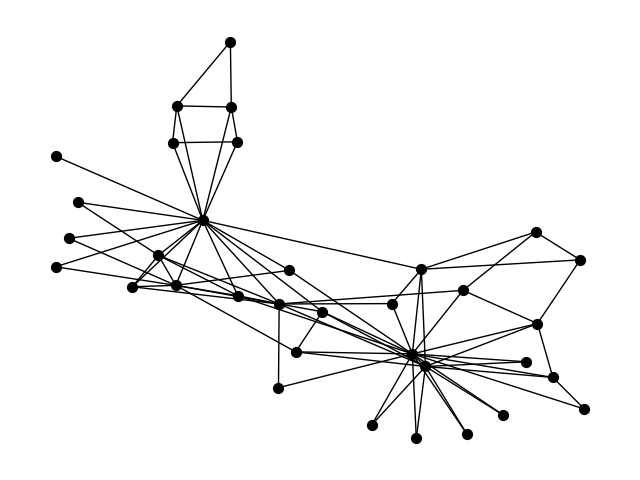
\includegraphics[width=\textwidth]{img/zachary_spring}
            \caption{Spring Layout.}
            \label{fig:zachary_spring}
        \end{subfigure}
        \begin{subfigure}[b]{0.45\textwidth}
            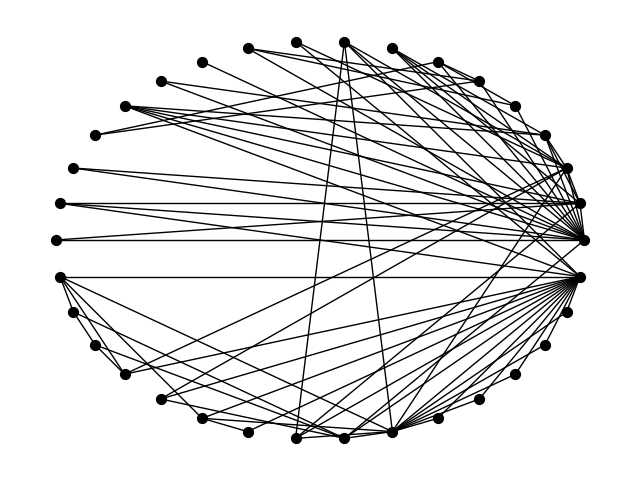
\includegraphics[width=\textwidth]{img/zachary_circle}
            \caption{Circle Layout.}
            \label{fig:zachary_circle}
        \end{subfigure}
    \end{center}
    \caption{Two renderings of the Zachary Karate Club network using data from KONECT.cc \cite{konect} and a Python library NetworkX \cite{SciPyProceedings_11}.}
    \label{fig:zachary_digrams}
\end{figure}

There exist different ways to represent social networks and the representation you choose depends on the question you are trying to answer. For example, one might imagine having two types of nodes in a network. One type of node will represent a person and another type of node will represent an event. An edge is drawn between a person and an event if a person attended a given event and person A is considered connected to person B if they both attended the same event. One such example of this is the \emph{Southern Women Dataset} \cite{konect:southernwomen}. This dataset is another example of a community detection problem because, after analysis of the network data, it was found that women in the group were split into two discrete subgroups. This is significant because it highlights that even without knowledge of how individuals interact at these events, we can still predict who they're likely to interact with.

\begin{figure}
    \begin{center}
        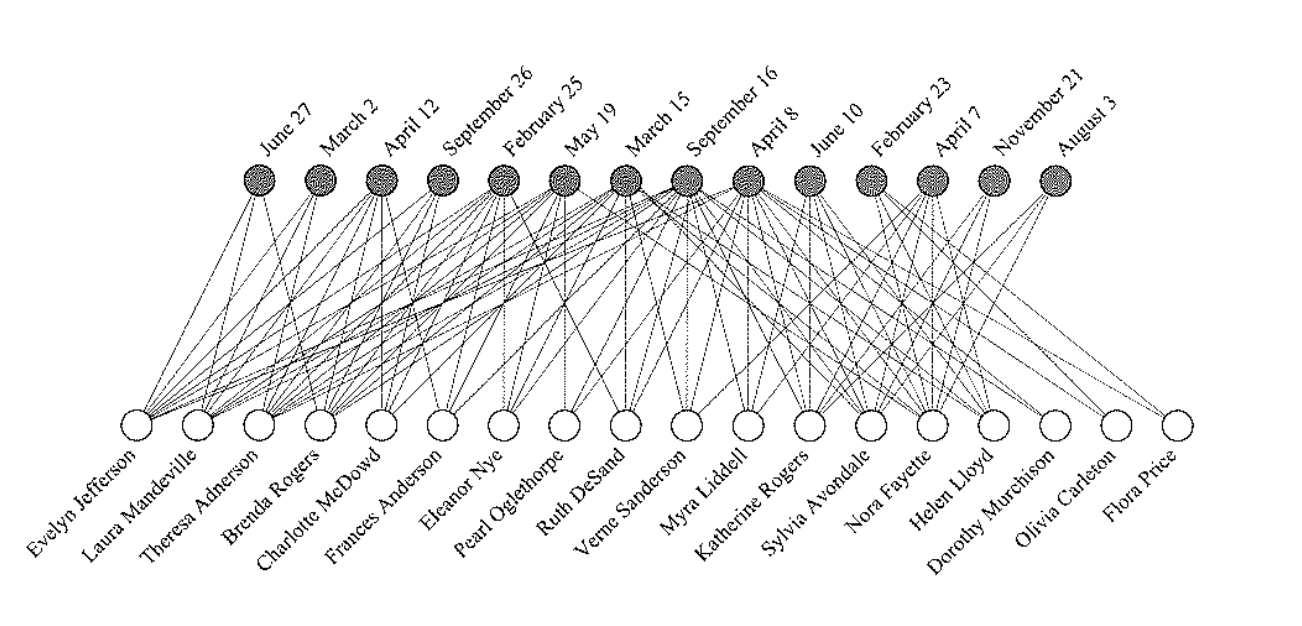
\includegraphics[width=0.95\textwidth]{img/southern_women}
    \end{center}
    \caption{A rendering of the Southern Women Dataset from Newman \cite[p. 39]{newman10}.}
    \label{fig:southernwomen}
\end{figure}

\subsection{Technological Networks}\label{sec:Technological Networks}
As a result of our intensely and digitally connected world, technological networks are of significant interest to researchers. The easiest example to consider is the Internet. The internet consists of many computers all connected by copper or fibre cables which signals are sent through to transmit data. As one might imagine, in the model, the computers are nodes and the cables are the edges. The internet needs to be robust against software and hardware failures and this is where the idea of community detection can help us. Saying that we want the internet to be robust is the same as saying that we want every node in the network to be strongly connected to every other node i.e. the number of possible routes between any two nodes is large. This means that, in the philosophy of community detection, we want the internet to act as one large community rather than multiple smaller communities that are loosely connected. An alternative way of looking at this is that once we've managed to identify the communities, we can then figure out which edges and nodes are the critical ones that allow passage from one community to another. This allows us to reinforce those edges and nodes to reduce the potential for failure.

Yet another example of a technological network would be the UK Power Grid. Network theory is a useful model here since for the UK Power Grid we're trying to solve exactly the same problem as with the internet --- we want the system to be robust against hardware or software failures. As such, identifying a community structure in the network would help us understand where the critical failure points are and what we need to reinforce to make the system robust.

\subsection{Information Networks}\label{sec:Information Networks}
The most accessible example of an information network is that which is generated by looking back through the citations on a paper recursively. If Paper A references Paper B, then we will draw a directed edge connecting Paper A to Paper B. This will generate a network that shows which papers are referenced by which other papers and how information is reused. Applying community detection to such a network would show us the different academic working groups and perhaps even different fields or subfields of a subject. An example of such an analysis is given by Redner \cite{Redner1998}.

Another example of an information network is the World Wide Web which differs from the internet in that it refers to the webpages hosted on the internet rather than the servers and cables themselves. Mapping the world wide web as a network shows us communities of websites that regularly reference each other. The idea of modelling the world wide web as a network has been used by companies like Google to develop tools like PageRank to enable easier browsing of the web \cite{pagerank} and it also allows us to get an understanding of the topology of the web as a whole \cite{BARABASI200069}.

Now that we're motivated to think about communities, we will move on to discussing the intricacies of the properties of networks that allow us to detect such structure before moving on to consider community detection methods and applications thereof.
